%%%%%%%%%%%%%%%%%%%%%%%%%%%%%%%%%%%%%%%%%%%%%%%%%%%%%%%%%%%%%%%%%%%%%%%%%%%%%%
%
% タイトル TeX用テンプレート 
% バージョン 2014-11-8 (Sat) 初版
% 作成者 Kouhei Ito
% 作成場所 野々市市中林 DeuxMKK
% 用途 2段組レポートの作成等
%
%%%%%%%%%%%%%%%%%%%%%%%%%%%%%%%%%%%%%%%%%%%%%%%%%%%%%%%%%%%%%%%%%%%%%%%%%%%%%%%%
%\documentclass[11pt,twocolumn]{jsarticle}
\documentclass[11pt]{jsarticle}
\usepackage[dvipdfmx]{graphicx}
\usepackage{amsmath,amssymb}
\usepackage{url}
\usepackage{nidanfloat}

%% 体裁

% ページレイアウト(A4:297 mm × 210 mm,1 インチ = 25.4 mm)
% http://www.biwako.shiga-u.ac.jp/sensei/kumazawa/tex/layout.html
% http://www.slis.tsukuba.ac.jp/~fujisawa.makoto.fu/cgi-bin/wiki/index.php?TeX%A5%E1%A5%E2#p61e1b46
% 上 20 mm,下 22 mm,左右 20 mm の余白設定
\setlength{\topmargin}{-20truemm}
\setlength{\headheight}{10truemm}
\setlength{\headsep}{4.6truemm}
\setlength{\textheight}{255truemm}
\setlength{\oddsidemargin}{-5.4truemm}
\setlength{\evensidemargin}{-5.4truemm}  % twoside オプション指定時のみ有効
\setlength{\textwidth}{170truemm}
% \setlength{\columnsep}{8truemm}
\setlength{\columnsep}{6truemm}


%%%%%%%%%%%%%%%%%%%%%%%%%%%%%%%%%%%%%%%%%%%%%%%%%%%%%%%%%%%%%%%%%%%%%%%%%%%%%%%%
\title{超低重心六輪独立懸架ローバの報告書}
\author{金沢工業高等専門学校 畠中和久}
\date{2015-3-31}
%%%%%%%%%%%%%%%%%%%%%%%%%%%%%%%%%%%%%%%%%%%%%%%%%%%%%%%%%%%%%%%%%%%%%%%%%%%%%%%%
\begin{document}
\maketitle
\begin{abstract}
自動走行するロボットには安定した走りと悪路での振動の小ささ、そしてコンパクトである事が大切になる。しかしホイールを大きくすると安定性はあるがコンパクトでない。今回参加するつくばチャレンジでは市街の走行だが、信号や路上など様々な状況に対して適切な対処が取れるロボットの開発が必要である。そこで今年は重心を低くすることで走行に安定性を持たせることを目的として六輪のローバー型ロボットを製作した。
%ボルダの振り子を用いて重力加速度を測定した.
%得られた値は,$g=9.80 \pm 0.02 [\textrm{m}/\textrm{sec}^2]$であった.
\end{abstract}

\tableofcontents
%%%%%%%%%%%%%%%%%%%%%%%%%%%%%%%%%%%%%%%%%%%%%%%%%%%%%%%%%%%%%%%%%%%%%%%%%%%%%%%%
\section{はじめに}
\subsection{研究の目的}
つくば市では毎年行われる「つくばチャレンジ」というロボットの大会がある。これはつくば市内の遊歩道等の実環境を、移動ロボットに自律走行させる技術チャレンジであり、地域と研究者が協力して行う、人間とロボットが共存する社会の実現のための先端的技術への挑戦である。自律移動ロボットは自分の位置を正確に測定し、次にどこまで移動するのかを判断する制御が必要不可欠である。しかし、制御に用いる機械は凸凹道の振動などの外乱によって発生するノイズが大きくなると誤作動を起こし自己位置を間違って計測する恐れがある。そこで、それを避けるため超低重心なロボットを製作しそのノイズをできる限り小さくすることを目的として”超低重心六輪独立懸架ローバ”を制作する。
\subsection{研究背景}
伊藤研究室ではロボットの制御を主な研究内容としている。そのためにもソフトウェアだけでなくハードウェアも必要になるので、つくばチャレンジに合わせた自律移動ロボットのハード製作の担当を請け負った。
\section{目的達成の手順}
\subsection{各部の設計}
\subsubsection{全体の概要図}
製作する”超低重心六輪独立懸架ローバー”(以下六輪ローバ)は低重心であるがゆえにロボットそのものが低く平らに長い長方形のようになる。そのままでは運搬時に非常に不便なため、モータを持つドライブモジュール(以下Dモジュール)と指示塔であるコントロールモジュール(以下Cモジュール)に分解できるように設計し、分解から組み立てを容易とするようにした。つまり2つのDモジュールからなる1つのロボットである(図\ref{fig:rokurin}参照)

\begin{figure}[htbt]
 \begin{center}
  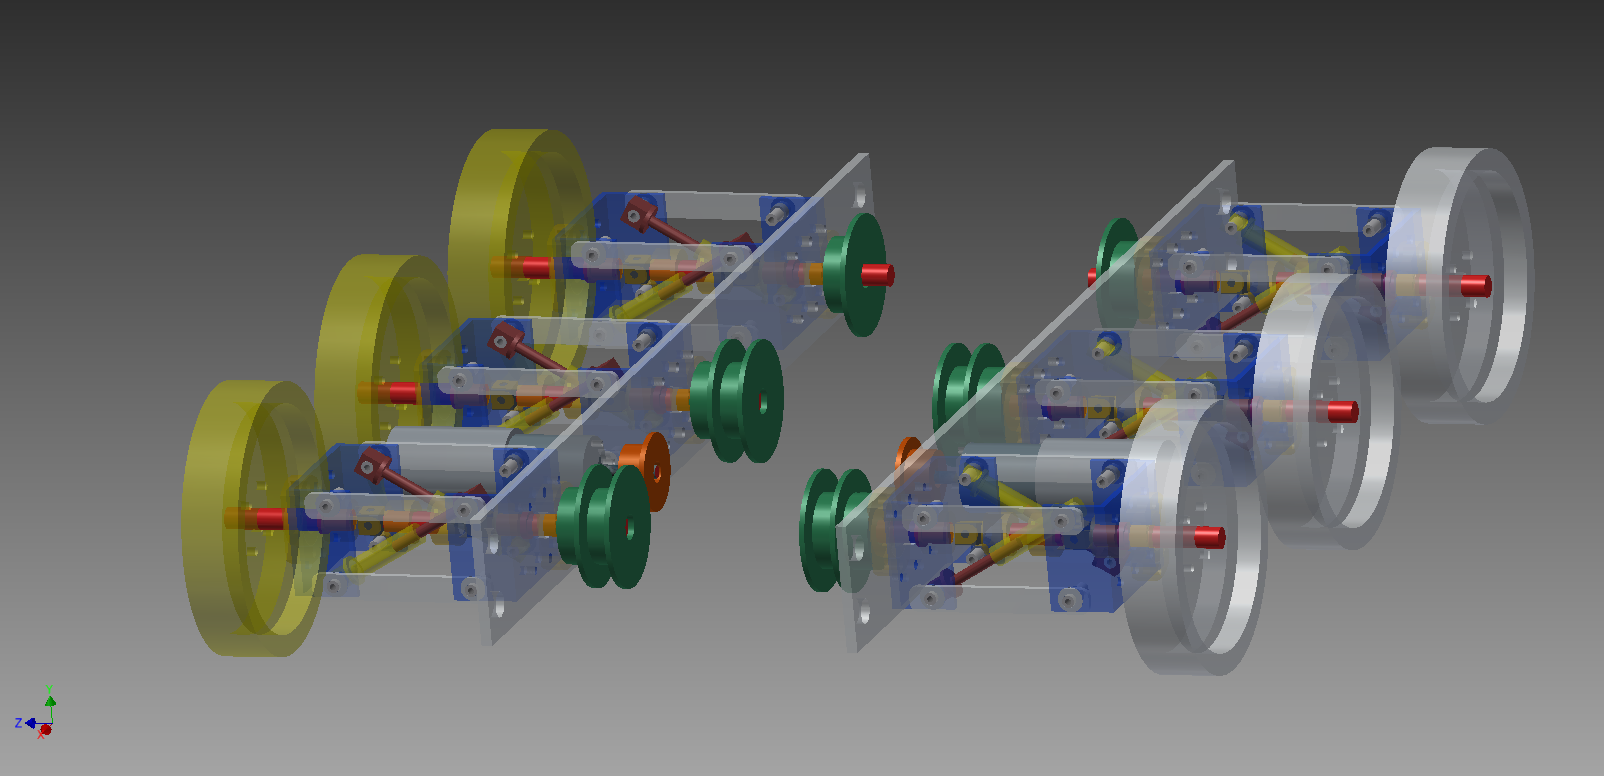
\includegraphics[width=100mm]{int.png}
  \caption{六輪ローバ}
  \label{fig:rokurin}%ここに文章中で使用する名前を指定する
 \end{center}
\end{figure}
\subsection{サスペンション}

設計したロボットはある程度の段差を超えるために車やミニ四駆のようなサスペンションを採用した(図\ref{fig:strat}参照)。しかし車やミニ四駆などに使用されるサスペンションはどれもストラット式サスペンションと呼ばれる各車輪が独立懸架するもので、部品点数が多くコストが高くなる。また設計するスペースの問題上、上昇するストロークも短い。しかし独立懸架は凸凹道を走行するには非常に適しているためこれを何とかしてコンパクトにまとめることが六輪ローバを開発する際に特に重要となった。その説明をこれから以下に示す。

\begin{figure}[htbt]
 \begin{center}
  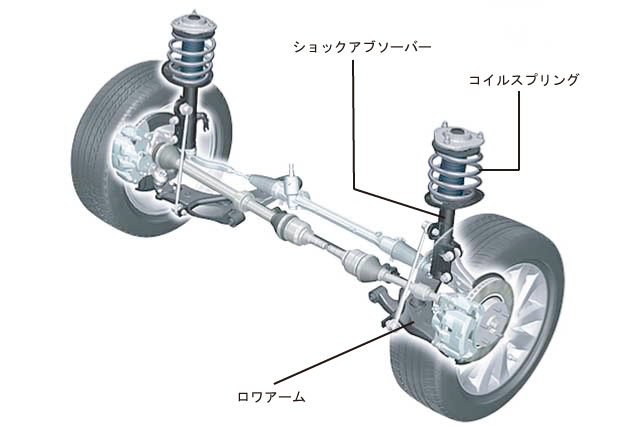
\includegraphics[width=120mm]{strat.jpg}
  \caption{ストラット式サスペンション}
  \label{fig:strat}%ここに文章中で使用する名前を指定する
 \end{center}
\end{figure}


\subsubsection{サスペンションの設計}
上記で示したように、ストラット式サスペンションは便利ではあるが問題点も目立つ。例えばストロークが少ない、ストロークを大きくすると車体が大きくなる、決められた場所にしか設置できない等で、「スペース」の点で問題が多いと考えた。そこで並行リンクとユニバーサルジョイント、車輪を用いて1つの「ボックス」を作り、その箱の両斜辺に2つ直接斜めに設置すれば車輪の径に左右されるものの従来のものよりスペースが少なく上下機構が得られるのではないかと考えた。(図(\ref{fig:box}参照))

\begin{figure}[htbt]
 \begin{center}
  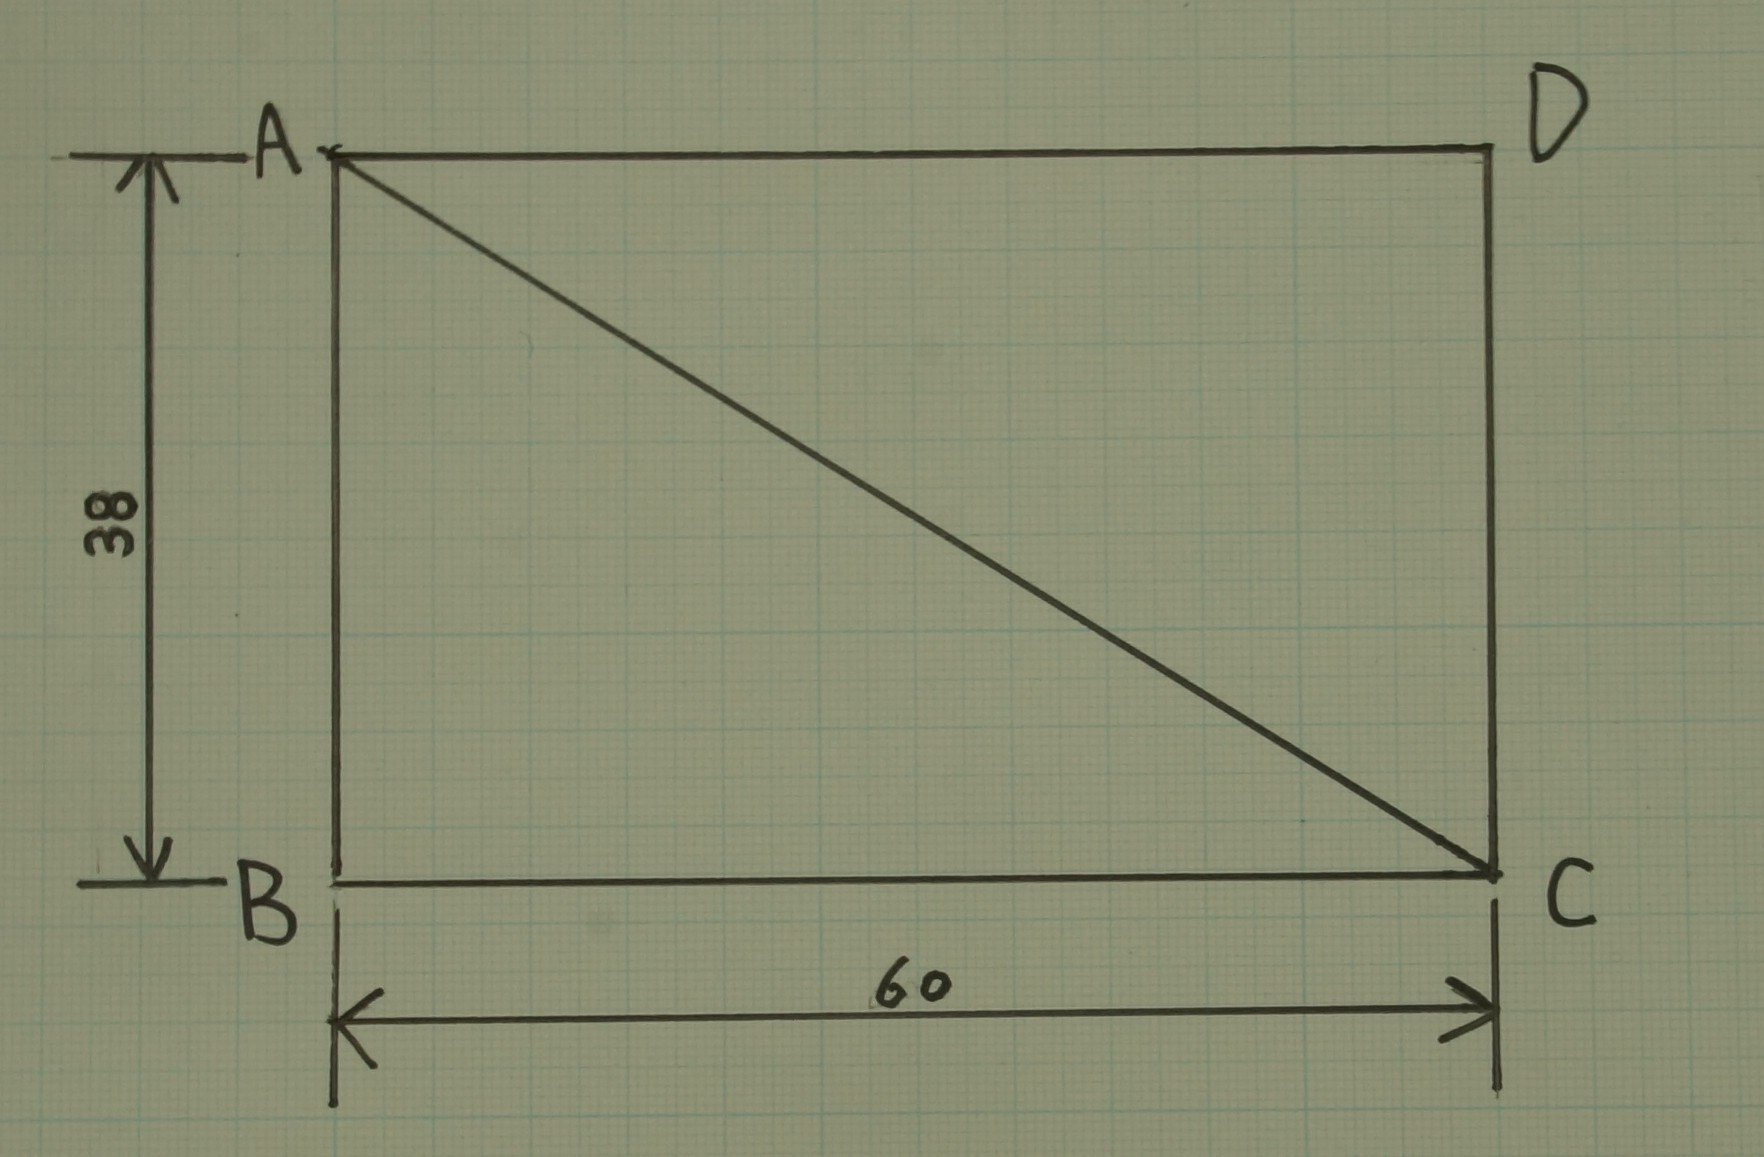
\includegraphics[width=60mm]{kanizu.jpg}
  \caption{ボックス}
  \label{fig:box}%ここに文章中で使用する名前を指定する
 \end{center}
\end{figure}






\subsubsection{箱の概要とサスペンションの配置}
以下に「ボックス」の製図を示す。また並行リンクが移動した際の図も示す(図\ref{fig:bix},\ref{fig:rink}参照)。これらの数値よりサスペンションのストロークと長さを求める。サスペンションの全体長さは斜辺に設置するため三平方の定理より
\begin{eqnarray}
   AC^2 & = & AB^2+CD^2 \\
  AC^2 & = & 38^2+60^2 = 71.022 ≒ 71.0 [mm]
\end{eqnarray}
となる。また今回は30[mm]程度の障害物を乗り越える想定しているため、このボックスの並行リンクが点A,Bを回転軸として点C,Dが30[mm]上昇した際の平行四辺形の斜辺を求める必要がある。並行リンクが移動してできるΔACEの斜辺AC'は
\begin{eqnarray}
   AC'^2 & = & AE^2+C'E^2 
\end{eqnarray}
となる。また辺AD'は辺BCと等しいので、辺AEは
\begin{eqnarray}
	AE^2 & = & AD'^2-D'E^2 \\
	AE^2 & = & 60^2-30^2 
\end{eqnarray}
となる。これを式(3)に代入すると斜辺AC2は
\begin{eqnarray}
	AC'^2 & = & AE^2+C'E^2 \\
	AC'^2 & = & (60^2-30^2)^2+(38-30)^2 ) \\
	AC' & = & 52.574 ≒ 52.6[mm]
\end{eqnarray}
となる。 \\
サスペンションは伸縮するものであり、それはこれらの辺ACと辺AC2の差分だけ変化することになる。今回の値から変化値x≒18.0[mm]ほどの変化があることが確定した。以上のAC,AC',xを用いてサスペンションの細かい設計を行う。



\begin{figure}[htbt]
 \begin{center}
  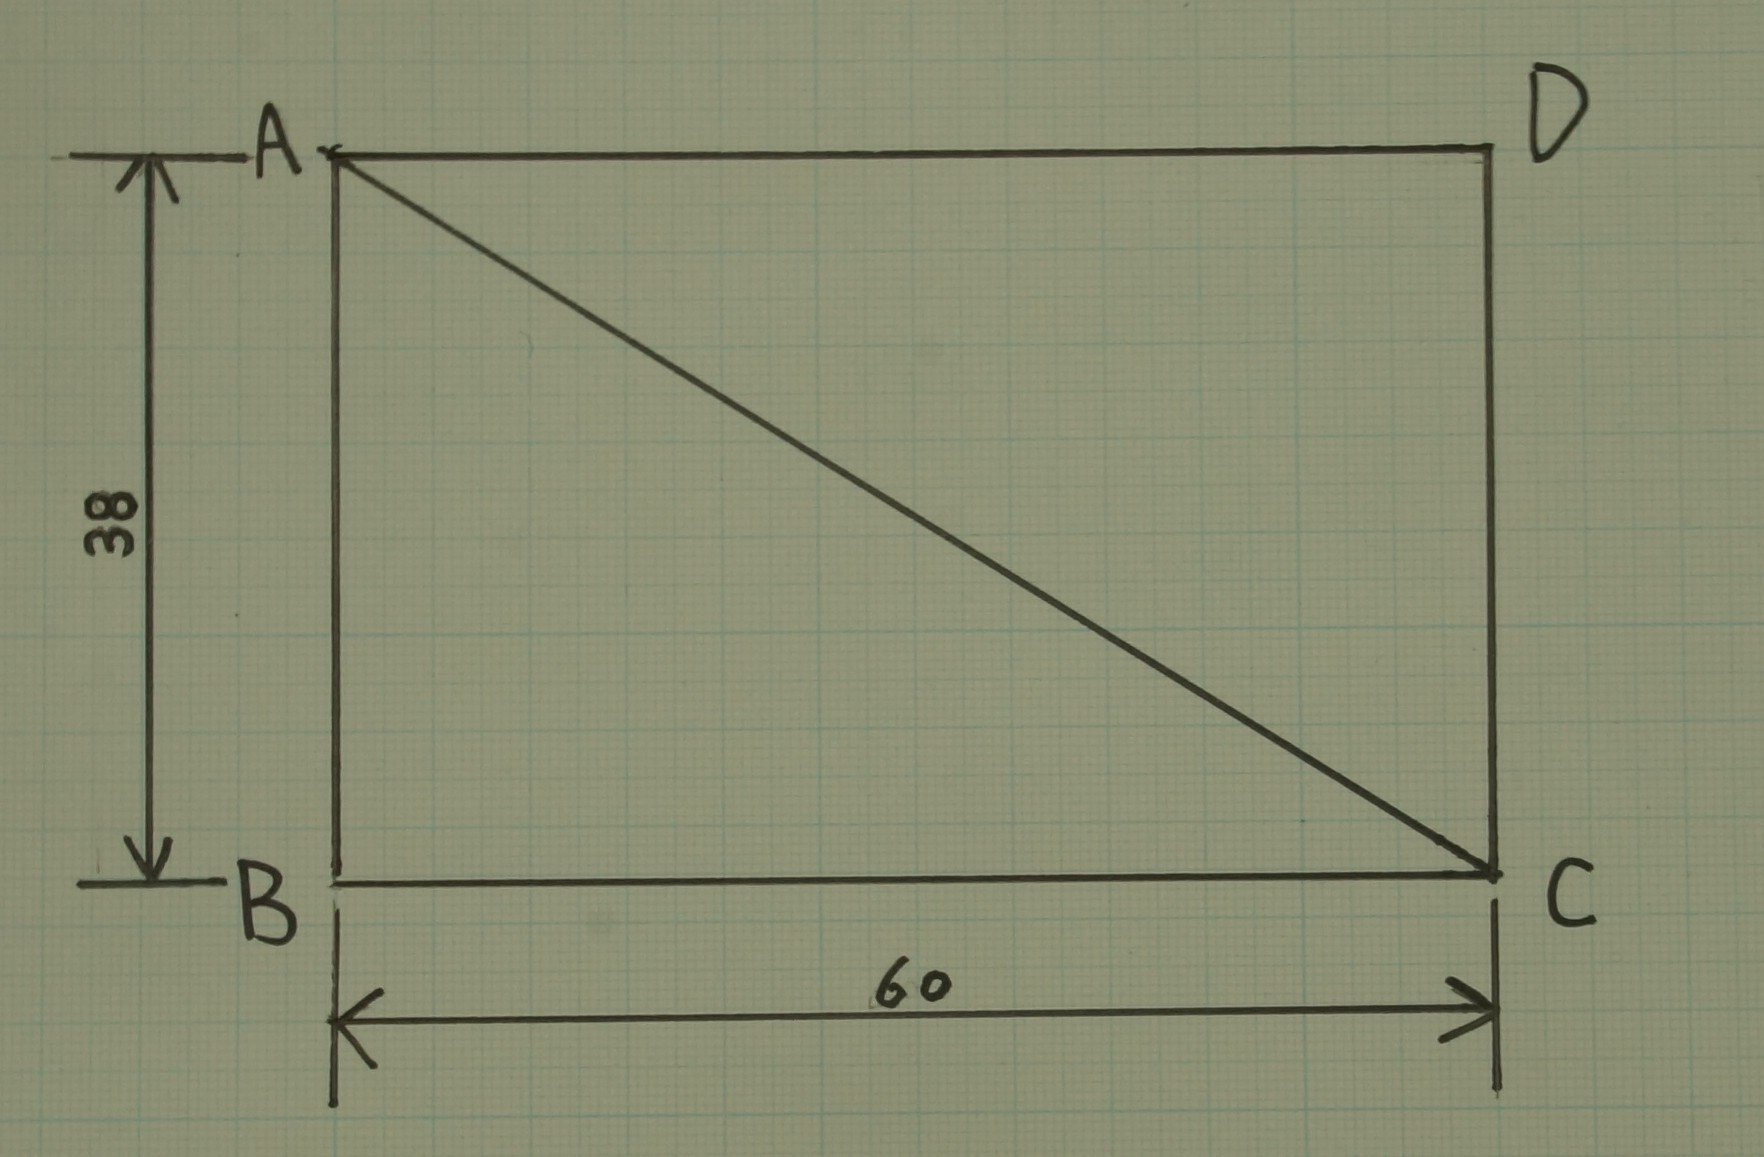
\includegraphics[width=60mm]{kanizu.jpg}
  \caption{ボックス}
  \label{fig:bix}%ここに文章中で使用する名前を指定する
 \end{center}
\end{figure}


\begin{figure}[htbt]
 \begin{center}
  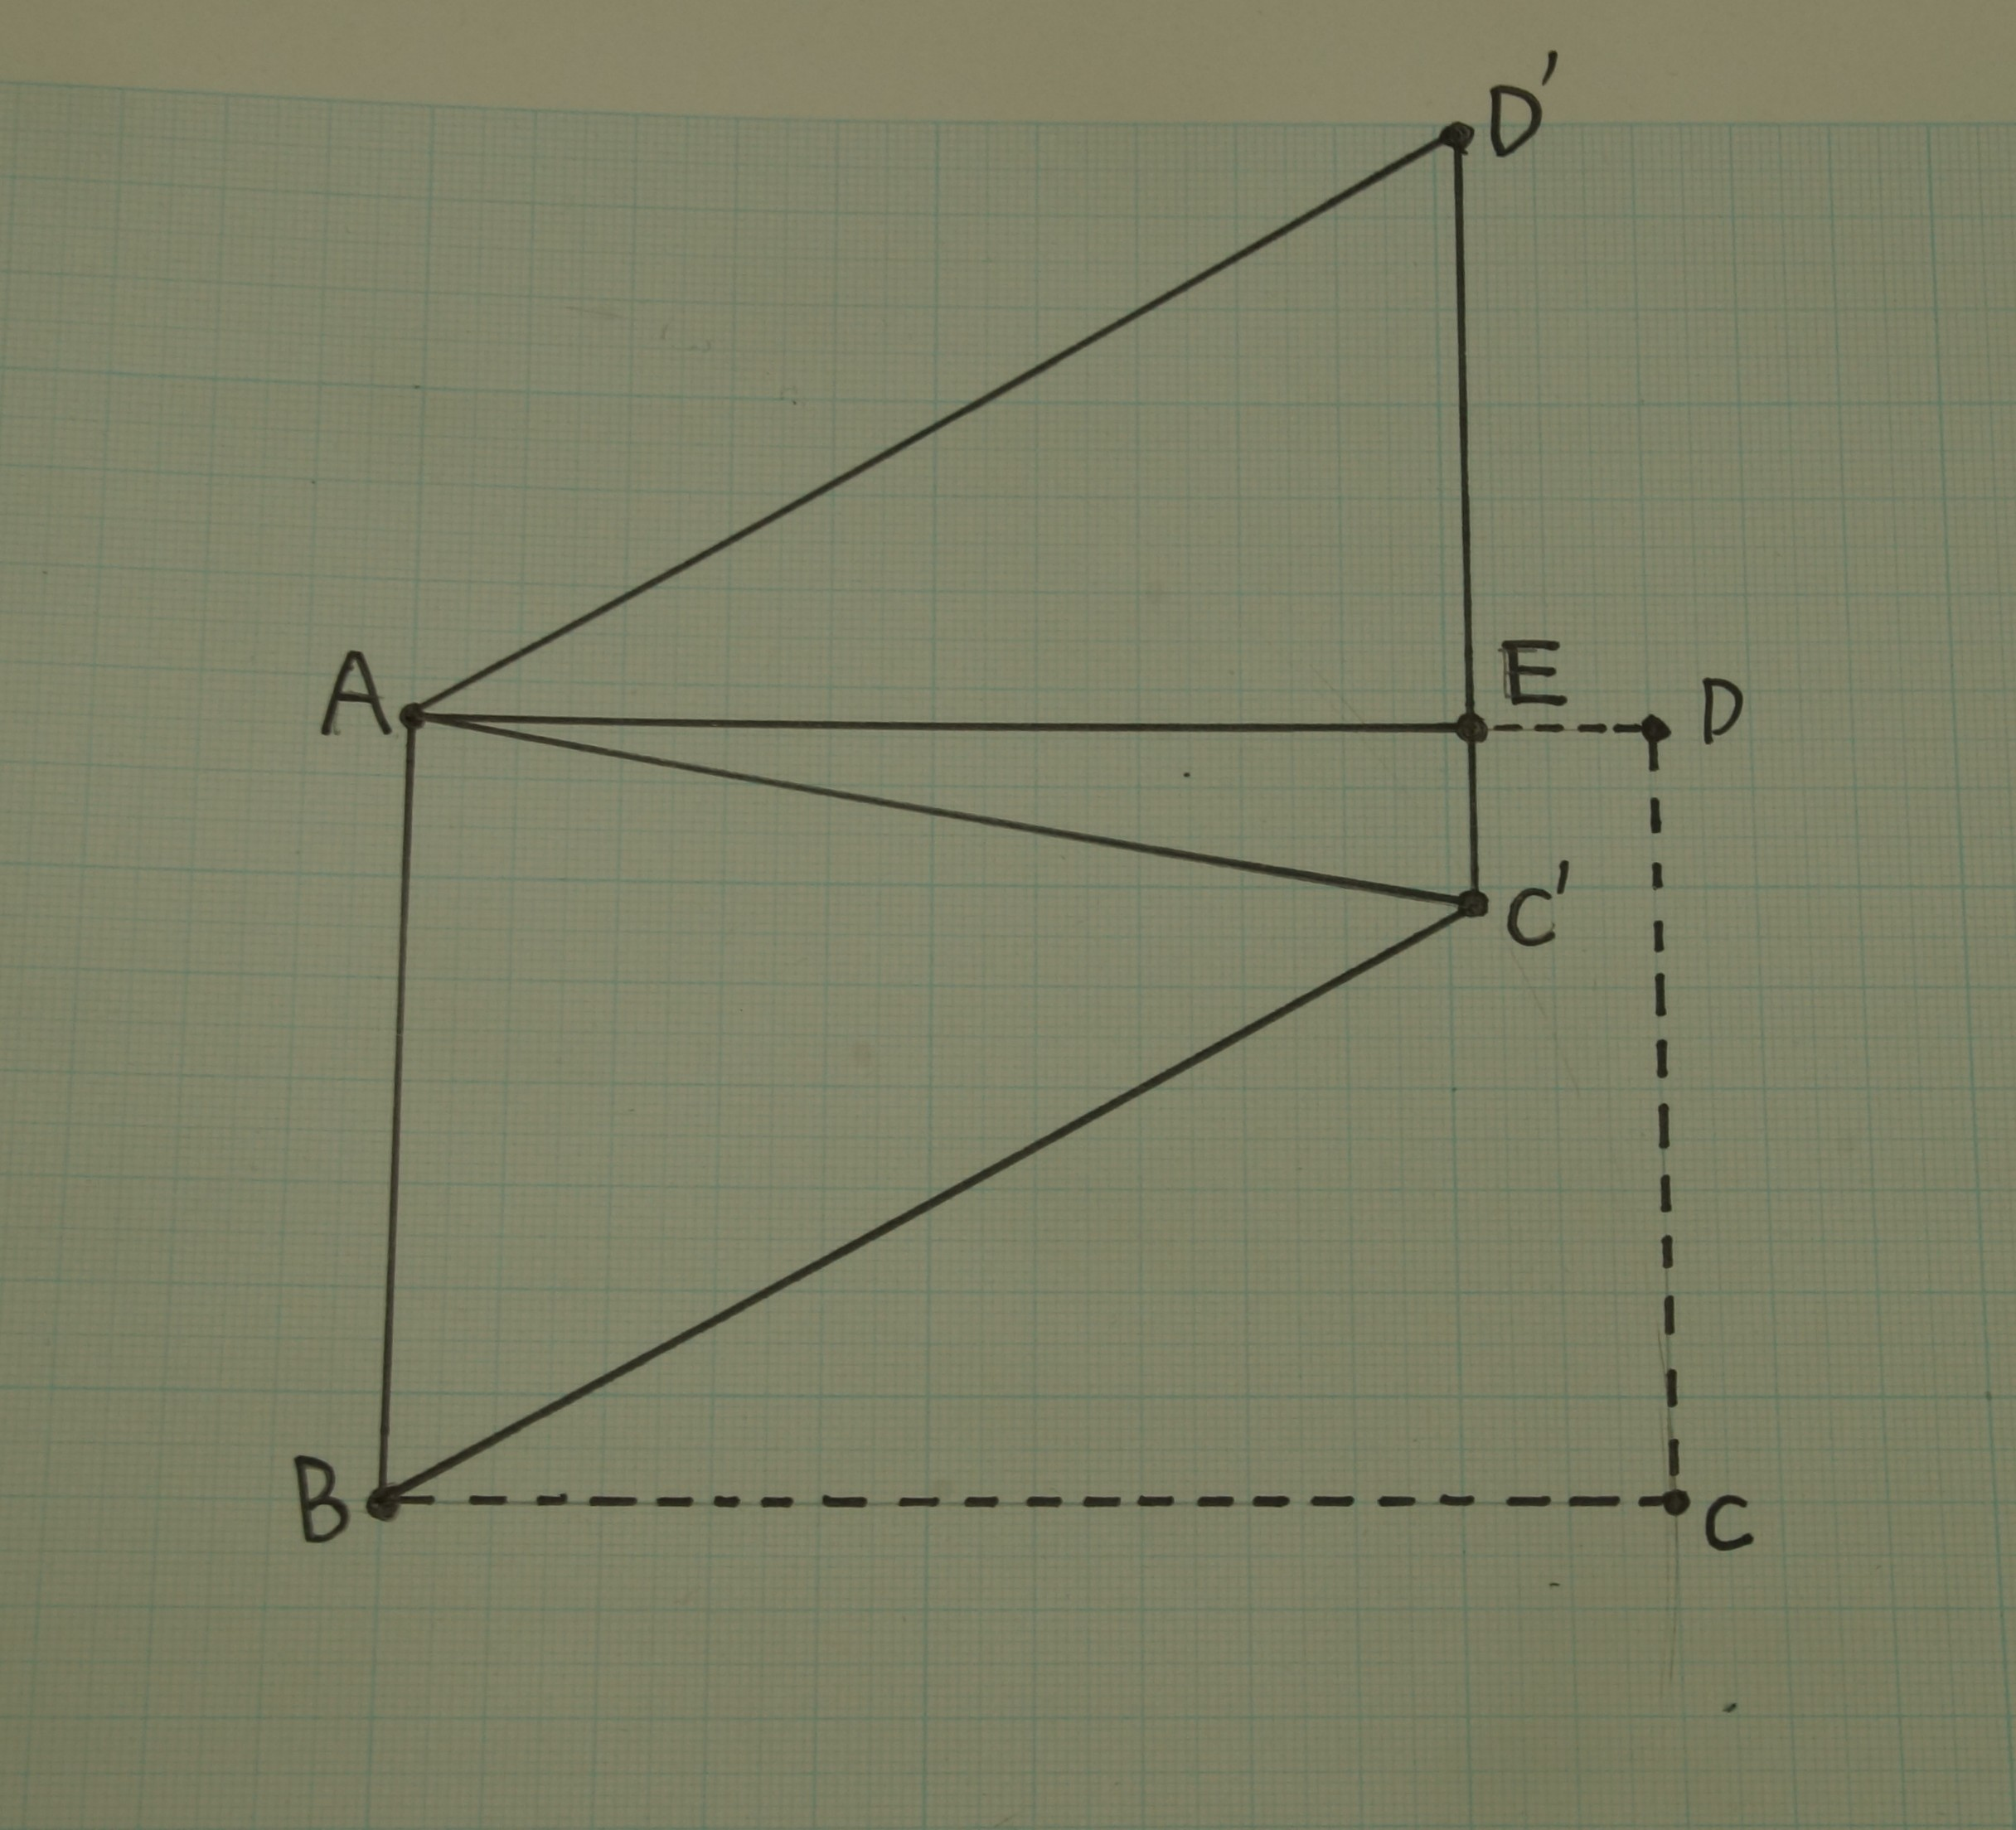
\includegraphics[width=60mm]{rink.jpg}
  \caption{平行リンクの移動量変化}
  \label{fig:rink}%ここに文章中で使用する名前を指定する
 \end{center}
\end{figure}








\subsubsection{サスペンションの設計}
サスペンションの大まかな大きさが判明したので細かい設計を行う。設計図を以下に示す(図\ref{fig:saspention}参照)。しかし、設計図を見ると分かったようにこのサスペンションにはショックアブソーバが取り付けられていないため、振動を吸収する機能がない。これではサスペンションにばねを取り付けても弾むだけで振動が抑えられないいので改善が必要である
\begin{figure}[htbt]
 \begin{center}
  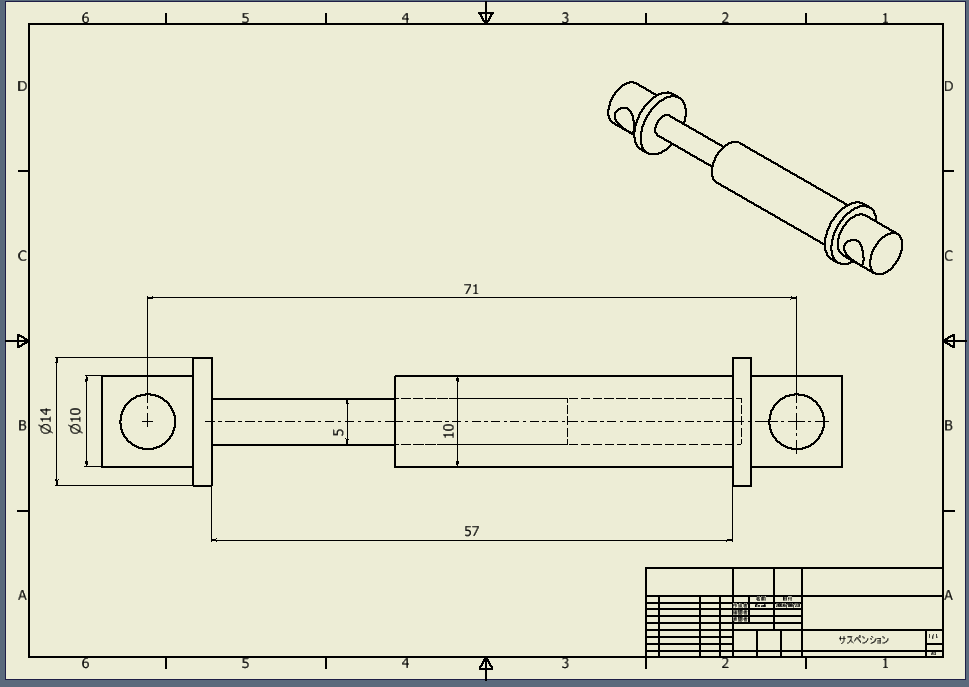
\includegraphics[width=120mm]{saspention.png}
  \caption{サスペンションの設計図}
  \label{fig:saspention}%ここに文章中で使用する名前を指定する
 \end{center}
\end{figure}




\subsection{サスペンションの力学計算}
サスペンションには路面の凹凸を車体に伝えない緩衝装置としての機能をもたせるため、ばねが必要であるため、フックの法則よりばねを選定する。そのためにばねにかかる力F[N]の式を求める。 \\
ボックスの点A,Bをそれぞれ固定支点と考えて計算を行う。図にFBDを示す。図よりx,y,Mの式はそれぞれ

\begin{eqnarray}
	x & = & R_AX+R_BX=0 \\
	y & = & R_AY+R_BY+F=0 \\
	M & = & BC・F-AB・R_AX=0
\end{eqnarray}
となる。更に点A,B,Cそれぞれの力のかかり方を求めると以下のようになる

\begin{figure}[htbt]
 \begin{center}
  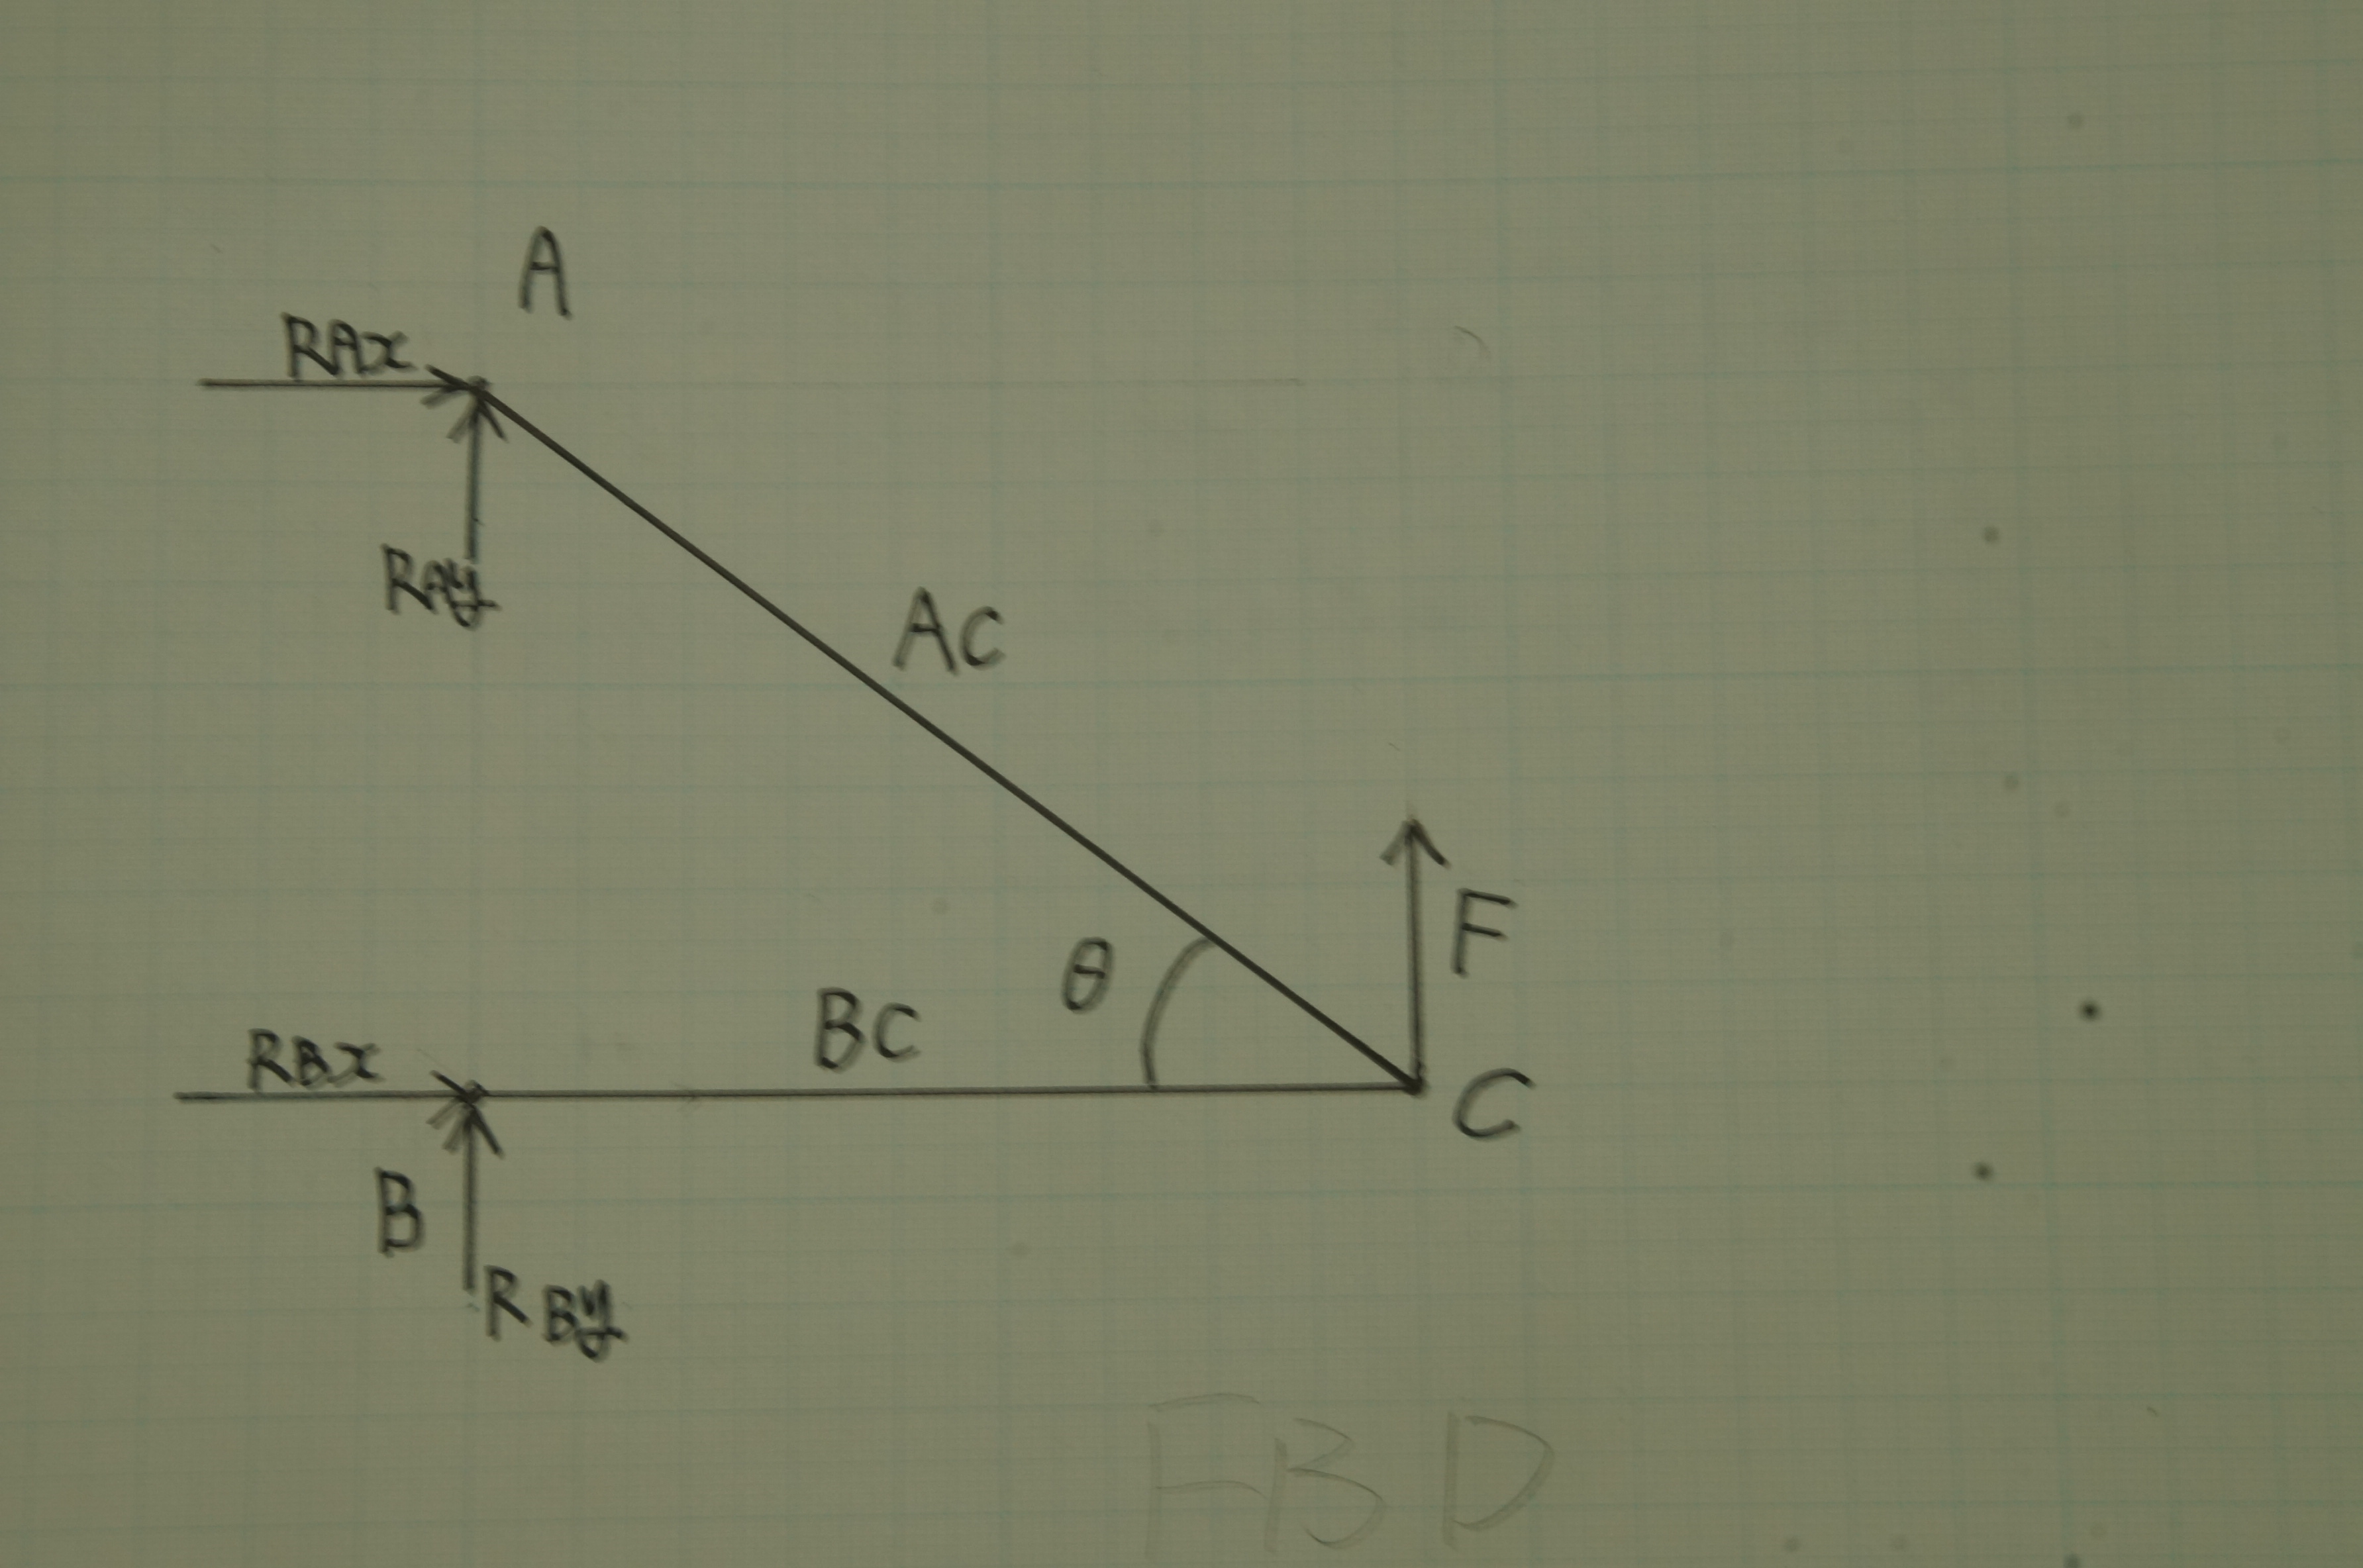
\includegraphics[width=100mm]{fbd.jpg}
  \caption{FBD}
  \label{fig:fbd}%ここに文章中で使用する名前を指定する
 \end{center}
\end{figure}

\subsubsection{点Aでの力学計算}
点Aでは図より以下のように計算できる。
\begin{eqnarray}
	R_AX+FAC・cosθ & = & 0 \\
	R_AY & = & FAC・sinθ 
\end{eqnarray}


\subsubsection{点Bでの力学計算}
点Bは図より以下のように計算できる。
\begin{eqnarray}
	R_BX+FBC & = & 0 \\
	R_BY & = & 0
\end{eqnarray}


\subsubsection{点Cでの力学計算}
点Cは図より以下のように計算できる。
\begin{eqnarray}
	FAC・cosθ+FBC & = & 0 \\
	F+FAC・sinθ & = & 0
\end{eqnarray}

\subsubsection{力学計算まとめ}
上記で求めた式より、FACにかかる力Fの式を計算する。
点Aと点Cより、FACにかかる力Fは
\begin{eqnarray}
	点A\\ R_AY+F & = & 0 \\
		F & = & -R_AY \\ 
		{これを代入すると} \\
	    R_AY & = & FAC・sinθ \\
		FAC & = & \frac{-F}{sinθ} [N] \\
		\\
	点C\\ F+FAD・sinθ & = & 0 \\
	FAC & = & \frac{-F}{sinθ} [N]
\end{eqnarray}

となることが確認できる。 \\
力FAC[N]はばね全体に掛る力なので、これをばね1個辺りに加わる力に除算する必要がある。今回作成する六輪ローバは一輪に2つのばねを持つため,ばねを合計で12個保有する。よってばね1個にかかる力FAC[N]は

\begin{eqnarray}
	FAC_12 & = & \frac{-F}{sinθ}*\frac{1}{12} [N] \\
\end{eqnarray}

となる。




\begin{figure}[htbt]
 \begin{center}
  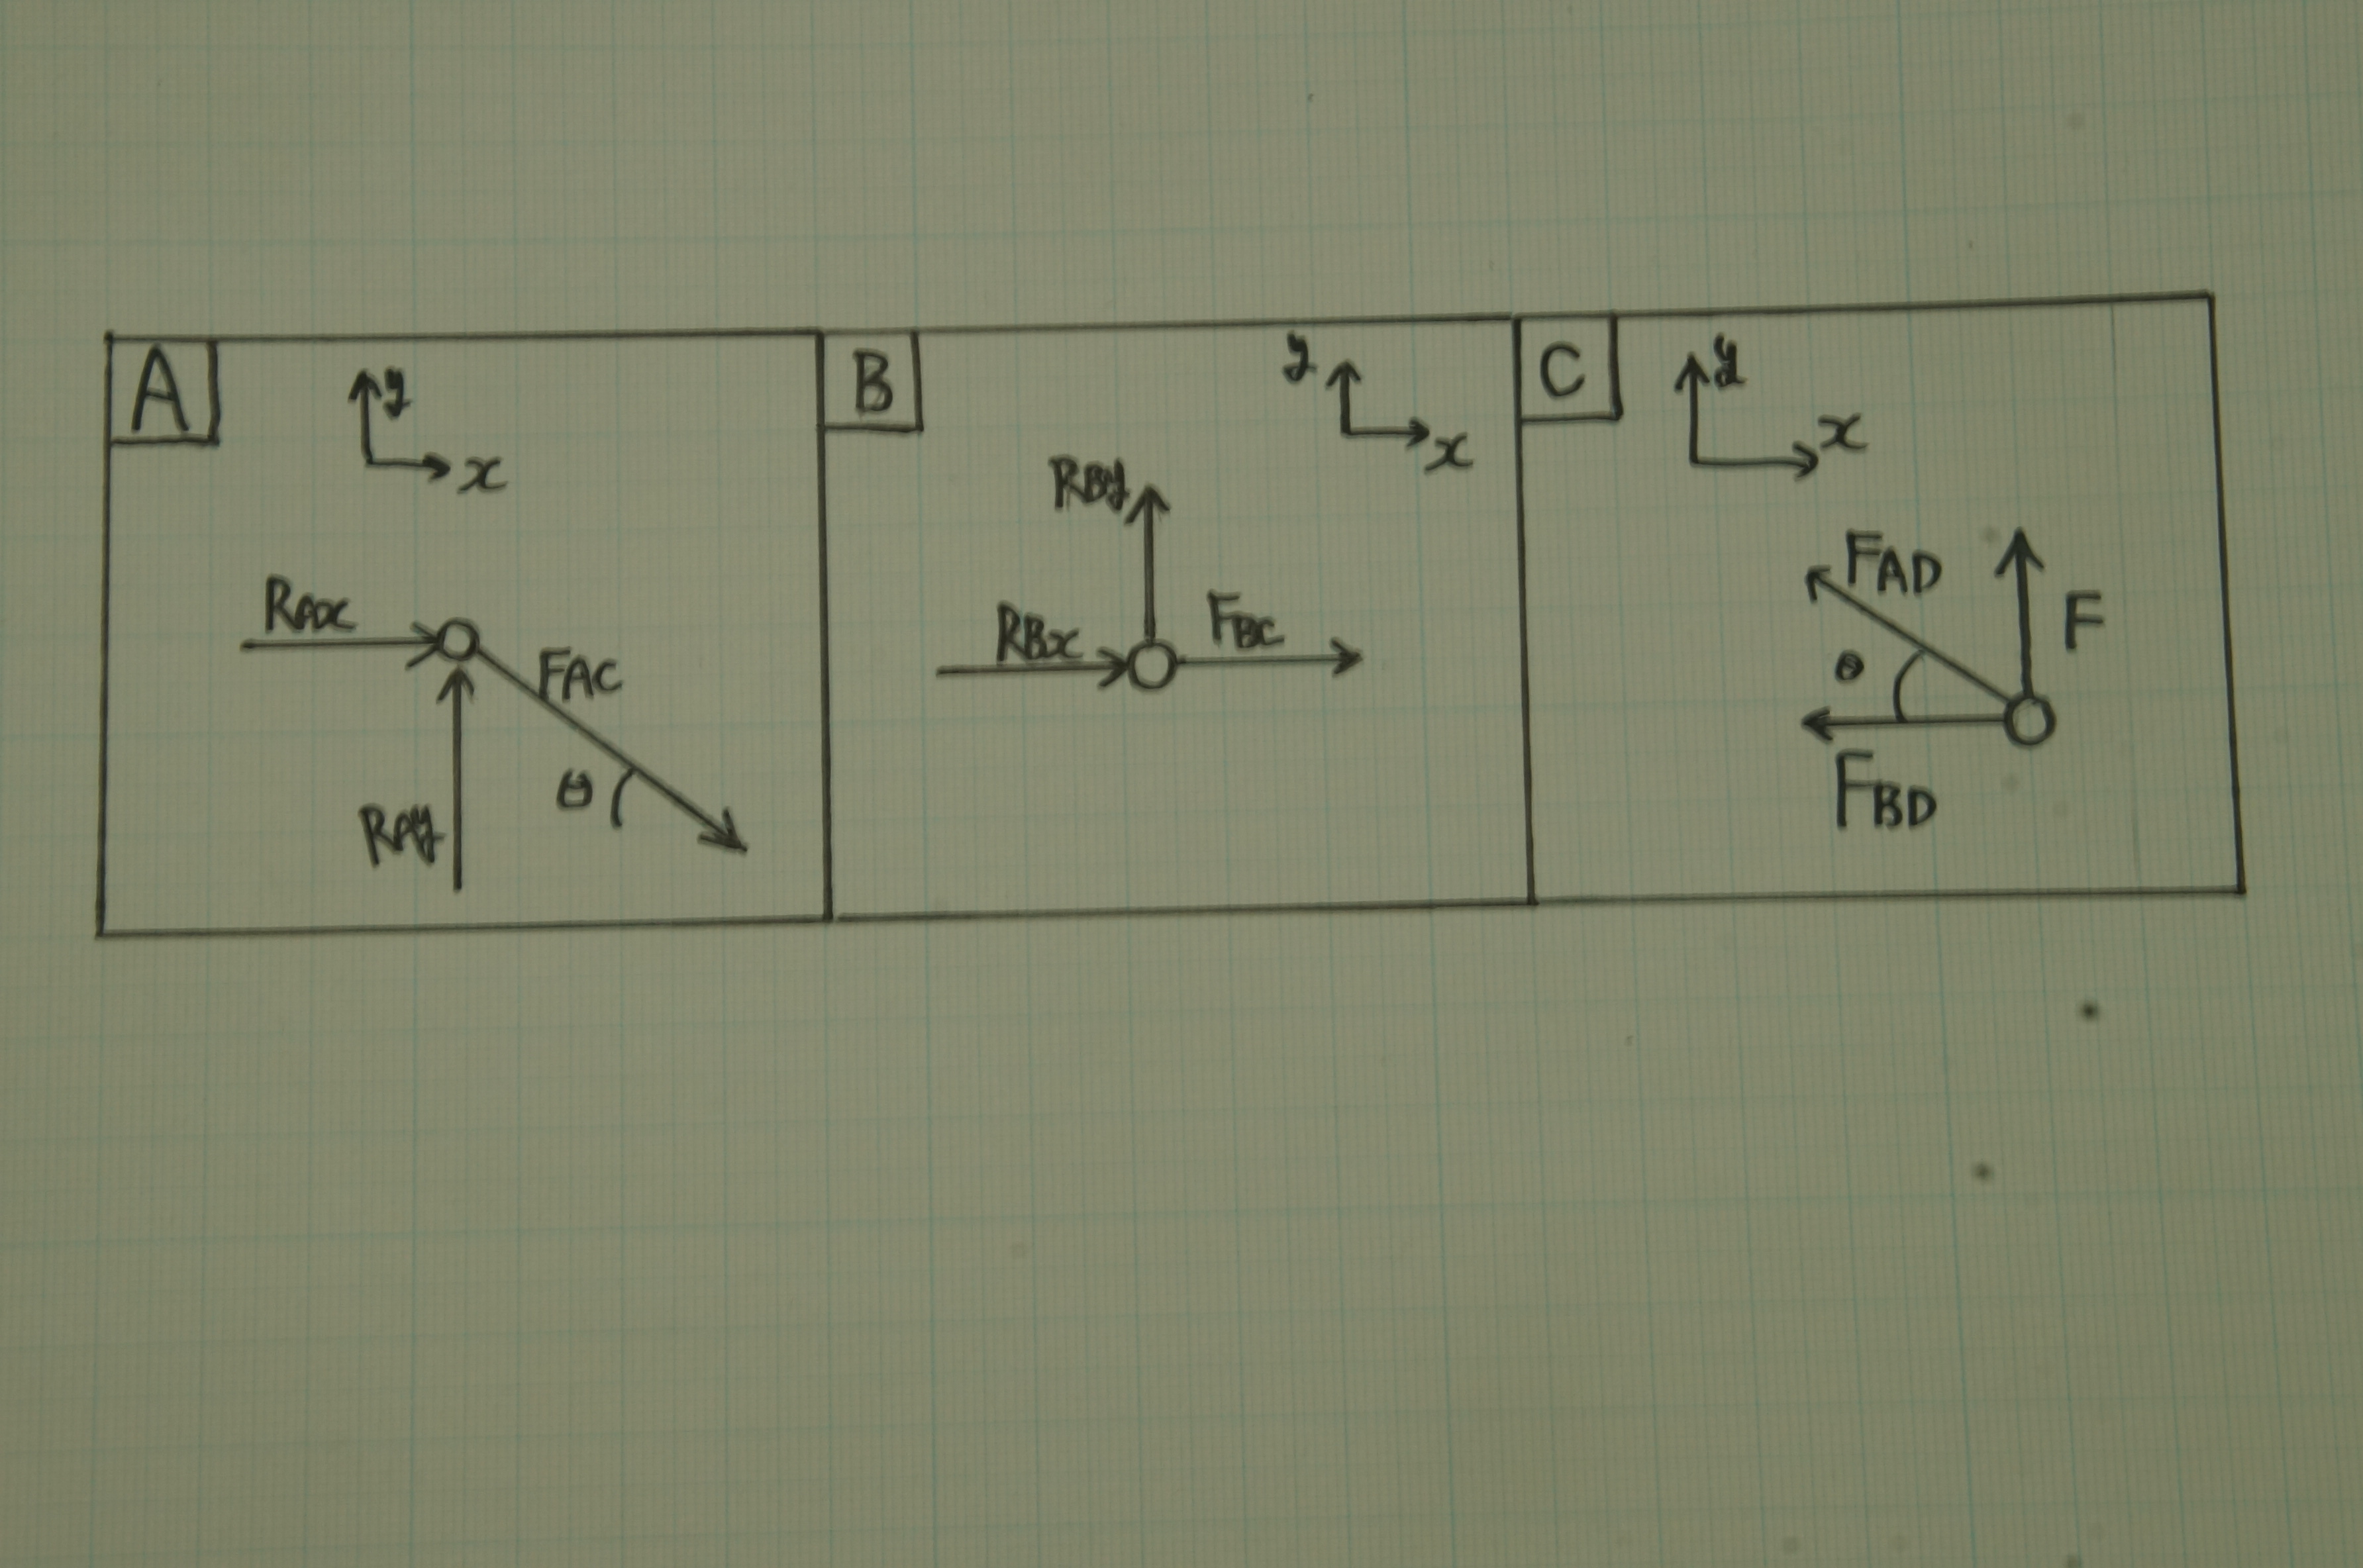
\includegraphics[width=100mm]{bai.jpg}
  \caption{各点にかかる力}
  \label{fig:bai}%ここに文章中で使用する名前を指定する
 \end{center}
\end{figure}





\section{考察}
このサスペンションが正常に機能するならば、つくば市街の道路を安定的に走行することが期待できる。しかし、本機体はサスペンションの超えられる障害物の想定を地元の道路から割り出しているため、大きな障害物に対しての性能は期待できない。



\end{document}
